\documentclass[1p]{elsarticle_modified}
%\bibliographystyle{elsarticle-num}

%\usepackage[colorlinks]{hyperref}
%\usepackage{abbrmath_seonhwa} %\Abb, \Ascr, \Acal ,\Abf, \Afrak
\usepackage{amsfonts}
\usepackage{amssymb}
\usepackage{amsmath}
\usepackage{amsthm}
\usepackage{scalefnt}
\usepackage{amsbsy}
\usepackage{kotex}
\usepackage{caption}
\usepackage{subfig}
\usepackage{color}
\usepackage{graphicx}
\usepackage{xcolor} %% white, black, red, green, blue, cyan, magenta, yellow
\usepackage{float}
\usepackage{setspace}
\usepackage{hyperref}

\usepackage{tikz}
\usetikzlibrary{arrows}

\usepackage{multirow}
\usepackage{array} % fixed length table
\usepackage{hhline}

%%%%%%%%%%%%%%%%%%%%%
\makeatletter
\renewcommand*\env@matrix[1][\arraystretch]{%
	\edef\arraystretch{#1}%
	\hskip -\arraycolsep
	\let\@ifnextchar\new@ifnextchar
	\array{*\c@MaxMatrixCols c}}
\makeatother %https://tex.stackexchange.com/questions/14071/how-can-i-increase-the-line-spacing-in-a-matrix
%%%%%%%%%%%%%%%

\usepackage[normalem]{ulem}

\newcommand{\msout}[1]{\ifmmode\text{\sout{\ensuremath{#1}}}\else\sout{#1}\fi}
%SOURCE: \msout is \stkout macro in https://tex.stackexchange.com/questions/20609/strikeout-in-math-mode

\newcommand{\cancel}[1]{
	\ifmmode
	{\color{red}\msout{#1}}
	\else
	{\color{red}\sout{#1}}
	\fi
}

\newcommand{\add}[1]{
	{\color{blue}\uwave{#1}}
}

\newcommand{\replace}[2]{
	\ifmmode
	{\color{red}\msout{#1}}{\color{blue}\uwave{#2}}
	\else
	{\color{red}\sout{#1}}{\color{blue}\uwave{#2}}
	\fi
}

\newcommand{\Sol}{\mathcal{S}} %segment
\newcommand{\D}{D} %diagram
\newcommand{\A}{\mathcal{A}} %arc


%%%%%%%%%%%%%%%%%%%%%%%%%%%%%5 test

\def\sl{\operatorname{\textup{SL}}(2,\Cbb)}
\def\psl{\operatorname{\textup{PSL}}(2,\Cbb)}
\def\quan{\mkern 1mu \triangleright \mkern 1mu}

\theoremstyle{definition}
\newtheorem{thm}{Theorem}[section]
\newtheorem{prop}[thm]{Proposition}
\newtheorem{lem}[thm]{Lemma}
\newtheorem{ques}[thm]{Question}
\newtheorem{cor}[thm]{Corollary}
\newtheorem{defn}[thm]{Definition}
\newtheorem{exam}[thm]{Example}
\newtheorem{rmk}[thm]{Remark}
\newtheorem{alg}[thm]{Algorithm}

\newcommand{\I}{\sqrt{-1}}
\begin{document}

%\begin{frontmatter}
%
%\title{Boundary parabolic representations of knots up to 8 crossings}
%
%%% Group authors per affiliation:
%\author{Yunhi Cho} 
%\address{Department of Mathematics, University of Seoul, Seoul, Korea}
%\ead{yhcho@uos.ac.kr}
%
%
%\author{Seonhwa Kim} %\fnref{s_kim}}
%\address{Center for Geometry and Physics, Institute for Basic Science, Pohang, 37673, Korea}
%\ead{ryeona17@ibs.re.kr}
%
%\author{Hyuk Kim}
%\address{Department of Mathematical Sciences, Seoul National University, Seoul 08826, Korea}
%\ead{hyukkim@snu.ac.kr}
%
%\author{Seokbeom Yoon}
%\address{Department of Mathematical Sciences, Seoul National University, Seoul, 08826,  Korea}
%\ead{sbyoon15@snu.ac.kr}
%
%\begin{abstract}
%We find all boundary parabolic representation of knots up to 8 crossings.
%
%\end{abstract}
%\begin{keyword}
%    \MSC[2010] 57M25 
%\end{keyword}
%
%\end{frontmatter}

%\linenumbers
%\tableofcontents
%
\newcommand\colored[1]{\textcolor{white}{\rule[-0.35ex]{0.8em}{1.4ex}}\kern-0.8em\color{red} #1}%
%\newcommand\colored[1]{\textcolor{white}{ #1}\kern-2.17ex	\textcolor{white}{ #1}\kern-1.81ex	\textcolor{white}{ #1}\kern-2.15ex\color{red}#1	}

{\Large $\underline{12n_{0716}~(K12n_{0716})}$}

\setlength{\tabcolsep}{10pt}
\renewcommand{\arraystretch}{1.6}
\vspace{1cm}\begin{tabular}{m{100pt}>{\centering\arraybackslash}m{274pt}}
\multirow{5}{120pt}{
	\centering
	\includegraphics[width=112pt]{../../../GIT/diagram.site/Diagrams/png/2805_12n_0716.png}\\
\ \ \ A knot diagram\footnotemark}&
\allowdisplaybreaks
\textbf{Linearized knot diagam} \\
\cline{2-2}
 &
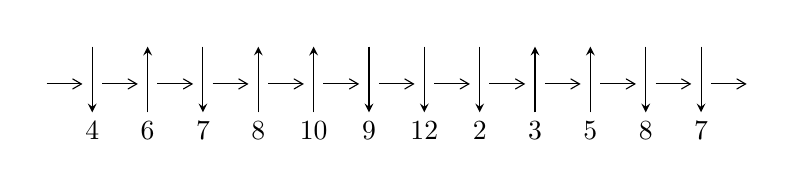
\begin{tikzpicture}[x=20pt, y=17pt]
	% nodes
	\node (C0) at (0, 0) {};
	\node (C1) at (1, 0) {};
	\node (C1U) at (1, +1) {};
	\node (C1D) at (1, -1) {4};

	\node (C2) at (2, 0) {};
	\node (C2U) at (2, +1) {};
	\node (C2D) at (2, -1) {6};

	\node (C3) at (3, 0) {};
	\node (C3U) at (3, +1) {};
	\node (C3D) at (3, -1) {7};

	\node (C4) at (4, 0) {};
	\node (C4U) at (4, +1) {};
	\node (C4D) at (4, -1) {8};

	\node (C5) at (5, 0) {};
	\node (C5U) at (5, +1) {};
	\node (C5D) at (5, -1) {10};

	\node (C6) at (6, 0) {};
	\node (C6U) at (6, +1) {};
	\node (C6D) at (6, -1) {9};

	\node (C7) at (7, 0) {};
	\node (C7U) at (7, +1) {};
	\node (C7D) at (7, -1) {12};

	\node (C8) at (8, 0) {};
	\node (C8U) at (8, +1) {};
	\node (C8D) at (8, -1) {2};

	\node (C9) at (9, 0) {};
	\node (C9U) at (9, +1) {};
	\node (C9D) at (9, -1) {3};

	\node (C10) at (10, 0) {};
	\node (C10U) at (10, +1) {};
	\node (C10D) at (10, -1) {5};

	\node (C11) at (11, 0) {};
	\node (C11U) at (11, +1) {};
	\node (C11D) at (11, -1) {8};

	\node (C12) at (12, 0) {};
	\node (C12U) at (12, +1) {};
	\node (C12D) at (12, -1) {7};
	\node (C13) at (13, 0) {};

	% arrows
	\draw[->,>={angle 60}]
	(C0) edge (C1) (C1) edge (C2) (C2) edge (C3) (C3) edge (C4) (C4) edge (C5) (C5) edge (C6) (C6) edge (C7) (C7) edge (C8) (C8) edge (C9) (C9) edge (C10) (C10) edge (C11) (C11) edge (C12) (C12) edge (C13) ;	\draw[->,>=stealth]
	(C1U) edge (C1D) (C2D) edge (C2U) (C3U) edge (C3D) (C4D) edge (C4U) (C5D) edge (C5U) (C6U) edge (C6D) (C7U) edge (C7D) (C8U) edge (C8D) (C9D) edge (C9U) (C10D) edge (C10U) (C11U) edge (C11D) (C12U) edge (C12D) ;
	\end{tikzpicture} \\
\hhline{~~} \\& 
\textbf{Solving Sequence} \\ \cline{2-2} 
 &
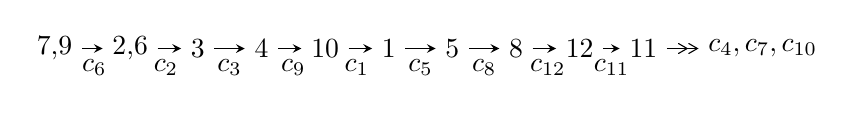
\begin{tikzpicture}[x=23pt, y=7pt]
	% node
	\node (A0) at (-1/8, 0) {7,9};
	\node (A1) at (17/16, 0) {2,6};
	\node (A2) at (17/8, 0) {3};
	\node (A3) at (25/8, 0) {4};
	\node (A4) at (33/8, 0) {10};
	\node (A5) at (41/8, 0) {1};
	\node (A6) at (49/8, 0) {5};
	\node (A7) at (57/8, 0) {8};
	\node (A8) at (65/8, 0) {12};
	\node (A9) at (73/8, 0) {11};
	\node (C1) at (1/2, -1) {$c_{6}$};
	\node (C2) at (13/8, -1) {$c_{2}$};
	\node (C3) at (21/8, -1) {$c_{3}$};
	\node (C4) at (29/8, -1) {$c_{9}$};
	\node (C5) at (37/8, -1) {$c_{1}$};
	\node (C6) at (45/8, -1) {$c_{5}$};
	\node (C7) at (53/8, -1) {$c_{8}$};
	\node (C8) at (61/8, -1) {$c_{12}$};
	\node (C9) at (69/8, -1) {$c_{11}$};
	\node (A10) at (11, 0) {$c_{4},c_{7},c_{10}$};

	% edge
	\draw[->,>=stealth]	
	(A0) edge (A1) (A1) edge (A2) (A2) edge (A3) (A3) edge (A4) (A4) edge (A5) (A5) edge (A6) (A6) edge (A7) (A7) edge (A8) (A8) edge (A9) ;
	\draw[->>,>={angle 60}]	
	(A9) edge (A10);
\end{tikzpicture} \\ 

\end{tabular} \\

\footnotetext{
The image of knot diagram is generated by the software ``\textbf{Draw programme}" developed by Andrew Bartholomew(\url{http://www.layer8.co.uk/maths/draw/index.htm\#Running-draw}), where we modified some parts for our purpose(\url{https://github.com/CATsTAILs/LinksPainter}).
}\phantom \\ \newline 
\centering \textbf{Ideals for irreducible components\footnotemark of $X_{\text{par}}$} 
 
\begin{align*}
I^u_{1}&=\langle 
9.32641\times10^{147} u^{57}-3.65205\times10^{146} u^{56}+\cdots+6.45245\times10^{146} b+1.05947\times10^{149},\\
\phantom{I^u_{1}}&\phantom{= \langle  }3.12608\times10^{148} u^{57}+1.49996\times10^{148} u^{56}+\cdots+6.45245\times10^{146} a+9.19957\times10^{149},\\
\phantom{I^u_{1}}&\phantom{= \langle  }u^{58}+u^{57}+\cdots+102 u+17\rangle \\
I^u_{2}&=\langle 
6502096368680 u^{18}+40798146932259 u^{17}+\cdots+25298539696097 b+12982884850055,\\
\phantom{I^u_{2}}&\phantom{= \langle  }-18835536785489 u^{18}-89002616845968 u^{17}+\cdots+25298539696097 a-49130182644029,\\
\phantom{I^u_{2}}&\phantom{= \langle  }u^{19}+4 u^{18}+\cdots-2 u+1\rangle \\
\\
\end{align*}
\raggedright * 2 irreducible components of $\dim_{\mathbb{C}}=0$, with total 77 representations.\\
\footnotetext{All coefficients of polynomials are rational numbers. But the coefficients are sometimes approximated in decimal forms when there is not enough margin.}
\newpage
\renewcommand{\arraystretch}{1}
\centering \section*{I. $I^u_{1}= \langle 9.33\times10^{147} u^{57}-3.65\times10^{146} u^{56}+\cdots+6.45\times10^{146} b+1.06\times10^{149},\;3.13\times10^{148} u^{57}+1.50\times10^{148} u^{56}+\cdots+6.45\times10^{146} a+9.20\times10^{149},\;u^{58}+u^{57}+\cdots+102 u+17 \rangle$}
\flushleft \textbf{(i) Arc colorings}\\
\begin{tabular}{m{7pt} m{180pt} m{7pt} m{180pt} }
\flushright $a_{7}=$&$\begin{pmatrix}1\\0\end{pmatrix}$ \\
\flushright $a_{9}=$&$\begin{pmatrix}0\\u\end{pmatrix}$ \\
\flushright $a_{2}=$&$\begin{pmatrix}-48.4480 u^{57}-23.2464 u^{56}+\cdots-6241.67 u-1425.75\\-14.4541 u^{57}+0.565994 u^{56}+\cdots-1020.45 u-164.197\end{pmatrix}$ \\
\flushright $a_{6}=$&$\begin{pmatrix}1\\- u^2\end{pmatrix}$ \\
\flushright $a_{3}=$&$\begin{pmatrix}-73.7734 u^{57}-30.7942 u^{56}+\cdots-9009.07 u-2018.38\\-2.48392 u^{57}+4.81221 u^{56}+\cdots+362.332 u+138.022\end{pmatrix}$ \\
\flushright $a_{4}=$&$\begin{pmatrix}-71.2895 u^{57}-35.6064 u^{56}+\cdots-9371.40 u-2156.40\\-2.48392 u^{57}+4.81221 u^{56}+\cdots+362.332 u+138.022\end{pmatrix}$ \\
\flushright $a_{10}=$&$\begin{pmatrix}-49.2274 u^{57}-16.9528 u^{56}+\cdots-5838.76 u-1396.24\\17.8595 u^{57}+6.03724 u^{56}+\cdots+2066.98 u+466.549\end{pmatrix}$ \\
\flushright $a_{1}=$&$\begin{pmatrix}87.3955 u^{57}+43.1083 u^{56}+\cdots+11436.3 u+2572.35\\-17.4932 u^{57}-11.0326 u^{56}+\cdots-2593.30 u-626.761\end{pmatrix}$ \\
\flushright $a_{5}=$&$\begin{pmatrix}-25.1085 u^{57}+7.32127 u^{56}+\cdots-879.198 u-1.92119\\13.8487 u^{57}+4.28606 u^{56}+\cdots+1443.05 u+285.809\end{pmatrix}$ \\
\flushright $a_{8}=$&$\begin{pmatrix}-38.4720 u^{57}-15.8661 u^{56}+\cdots-4872.65 u-1186.00\\8.37163 u^{57}+3.81598 u^{56}+\cdots+1075.83 u+256.175\end{pmatrix}$ \\
\flushright $a_{12}=$&$\begin{pmatrix}69.9024 u^{57}+32.0757 u^{56}+\cdots+8843.00 u+1945.59\\-17.4932 u^{57}-11.0326 u^{56}+\cdots-2593.30 u-626.761\end{pmatrix}$ \\
\flushright $a_{11}=$&$\begin{pmatrix}188.771 u^{57}+57.7574 u^{56}+\cdots+20419.4 u+4195.36\\-55.5034 u^{57}-26.6276 u^{56}+\cdots-7148.10 u-1617.81\end{pmatrix}$\\&\end{tabular}
\flushleft \textbf{(ii) Obstruction class $= -1$}\\~\\
\flushleft \textbf{(iii) Cusp Shapes $= 152.678 u^{57}+38.4757 u^{56}+\cdots+15871.4 u+3232.62$}\\~\\
\newpage\renewcommand{\arraystretch}{1}
\flushleft \textbf{(iv) u-Polynomials at the component}\newline \\
\begin{tabular}{m{50pt}|m{274pt}}
Crossings & \hspace{64pt}u-Polynomials at each crossing \\
\hline $$\begin{aligned}c_{1}\end{aligned}$$&$\begin{aligned}
&u^{58}+4 u^{57}+\cdots+36890 u+11033
\end{aligned}$\\
\hline $$\begin{aligned}c_{2}\end{aligned}$$&$\begin{aligned}
&u^{58}-3 u^{57}+\cdots+14 u+29
\end{aligned}$\\
\hline $$\begin{aligned}c_{3}\end{aligned}$$&$\begin{aligned}
&u^{58}- u^{57}+\cdots+3040 u+373
\end{aligned}$\\
\hline $$\begin{aligned}c_{4}\end{aligned}$$&$\begin{aligned}
&u^{58}- u^{57}+\cdots-79133 u+6037
\end{aligned}$\\
\hline $$\begin{aligned}c_{5},c_{10}\end{aligned}$$&$\begin{aligned}
&u^{58}- u^{57}+\cdots+226 u+299
\end{aligned}$\\
\hline $$\begin{aligned}c_{6}\end{aligned}$$&$\begin{aligned}
&u^{58}- u^{57}+\cdots-102 u+17
\end{aligned}$\\
\hline $$\begin{aligned}c_{7},c_{11},c_{12}\end{aligned}$$&$\begin{aligned}
&u^{58}- u^{56}+\cdots-77 u+67
\end{aligned}$\\
\hline $$\begin{aligned}c_{8}\end{aligned}$$&$\begin{aligned}
&u^{58}- u^{57}+\cdots-318 u+37
\end{aligned}$\\
\hline $$\begin{aligned}c_{9}\end{aligned}$$&$\begin{aligned}
&u^{58}- u^{57}+\cdots+597 u+301
\end{aligned}$\\
\hline
\end{tabular}\\~\\
\newpage\renewcommand{\arraystretch}{1}
\flushleft \textbf{(v) Riley Polynomials at the component}\newline \\
\begin{tabular}{m{50pt}|m{274pt}}
Crossings & \hspace{64pt}Riley Polynomials at each crossing \\
\hline $$\begin{aligned}c_{1}\end{aligned}$$&$\begin{aligned}
&y^{58}-70 y^{57}+\cdots+4940625850 y+121727089
\end{aligned}$\\
\hline $$\begin{aligned}c_{2}\end{aligned}$$&$\begin{aligned}
&y^{58}+11 y^{57}+\cdots+23062 y+841
\end{aligned}$\\
\hline $$\begin{aligned}c_{3}\end{aligned}$$&$\begin{aligned}
&y^{58}-67 y^{57}+\cdots-4505246 y+139129
\end{aligned}$\\
\hline $$\begin{aligned}c_{4}\end{aligned}$$&$\begin{aligned}
&y^{58}+97 y^{57}+\cdots-269971117 y+36445369
\end{aligned}$\\
\hline $$\begin{aligned}c_{5},c_{10}\end{aligned}$$&$\begin{aligned}
&y^{58}+77 y^{57}+\cdots+6195034 y+89401
\end{aligned}$\\
\hline $$\begin{aligned}c_{6}\end{aligned}$$&$\begin{aligned}
&y^{58}-7 y^{57}+\cdots-11084 y+289
\end{aligned}$\\
\hline $$\begin{aligned}c_{7},c_{11},c_{12}\end{aligned}$$&$\begin{aligned}
&y^{58}-2 y^{57}+\cdots-22277 y+4489
\end{aligned}$\\
\hline $$\begin{aligned}c_{8}\end{aligned}$$&$\begin{aligned}
&y^{58}-13 y^{57}+\cdots-27050 y+1369
\end{aligned}$\\
\hline $$\begin{aligned}c_{9}\end{aligned}$$&$\begin{aligned}
&y^{58}+39 y^{57}+\cdots+3573447 y+90601
\end{aligned}$\\
\hline
\end{tabular}\\~\\
\newpage\flushleft \textbf{(vi) Complex Volumes and Cusp Shapes}
$$\begin{array}{c|c|c}  
\text{Solutions to }I^u_{1}& \I (\text{vol} + \sqrt{-1}CS) & \text{Cusp shape}\\
 \hline 
\begin{aligned}
u &= \phantom{-}0.978354 + 0.283113 I \\
a &= -1.022500 - 0.316283 I \\
b &= \phantom{-}2.12647 + 2.00443 I\end{aligned}
 & -13.17140 + 2.12358 I & \phantom{-0.000000 } 0 \\ \hline\begin{aligned}
u &= \phantom{-}0.978354 - 0.283113 I \\
a &= -1.022500 + 0.316283 I \\
b &= \phantom{-}2.12647 - 2.00443 I\end{aligned}
 & -13.17140 - 2.12358 I & \phantom{-0.000000 } 0 \\ \hline\begin{aligned}
u &= -0.752867 + 0.705964 I \\
a &= -1.47988 + 0.29568 I \\
b &= \phantom{-}0.711075 - 0.693834 I\end{aligned}
 & \phantom{-}2.00803 + 4.95664 I & \phantom{-0.000000 } 0 \\ \hline\begin{aligned}
u &= -0.752867 - 0.705964 I \\
a &= -1.47988 - 0.29568 I \\
b &= \phantom{-}0.711075 + 0.693834 I\end{aligned}
 & \phantom{-}2.00803 - 4.95664 I & \phantom{-0.000000 } 0 \\ \hline\begin{aligned}
u &= -0.021606 + 1.042490 I \\
a &= \phantom{-}0.605699 - 0.199313 I \\
b &= -0.087128 - 0.351024 I\end{aligned}
 & -1.04699 - 2.20023 I & \phantom{-0.000000 } 0 \\ \hline\begin{aligned}
u &= -0.021606 - 1.042490 I \\
a &= \phantom{-}0.605699 + 0.199313 I \\
b &= -0.087128 + 0.351024 I\end{aligned}
 & -1.04699 + 2.20023 I & \phantom{-0.000000 } 0 \\ \hline\begin{aligned}
u &= \phantom{-}0.730237 + 0.516053 I \\
a &= \phantom{-}0.945824 - 0.083393 I \\
b &= -0.608386 - 0.180858 I\end{aligned}
 & -1.28329 - 0.82809 I & \phantom{-0.000000 } 0 \\ \hline\begin{aligned}
u &= \phantom{-}0.730237 - 0.516053 I \\
a &= \phantom{-}0.945824 + 0.083393 I \\
b &= -0.608386 + 0.180858 I\end{aligned}
 & -1.28329 + 0.82809 I & \phantom{-0.000000 } 0 \\ \hline\begin{aligned}
u &= -1.011420 + 0.459011 I \\
a &= \phantom{-}1.005890 + 0.081651 I \\
b &= -1.98236 - 0.47508 I\end{aligned}
 & -8.23668 + 4.75000 I & \phantom{-0.000000 } 0 \\ \hline\begin{aligned}
u &= -1.011420 - 0.459011 I \\
a &= \phantom{-}1.005890 - 0.081651 I \\
b &= -1.98236 + 0.47508 I\end{aligned}
 & -8.23668 - 4.75000 I & \phantom{-0.000000 } 0\\
 \hline 
 \end{array}$$\newpage$$\begin{array}{c|c|c}  
\text{Solutions to }I^u_{1}& \I (\text{vol} + \sqrt{-1}CS) & \text{Cusp shape}\\
 \hline 
\begin{aligned}
u &= -0.808030 + 0.355010 I \\
a &= -1.248830 + 0.214250 I \\
b &= \phantom{-}2.12302 - 1.95955 I\end{aligned}
 & -12.9566 + 6.6659 I & -8.33432 - 5.93696 I \\ \hline\begin{aligned}
u &= -0.808030 - 0.355010 I \\
a &= -1.248830 - 0.214250 I \\
b &= \phantom{-}2.12302 + 1.95955 I\end{aligned}
 & -12.9566 - 6.6659 I & -8.33432 + 5.93696 I \\ \hline\begin{aligned}
u &= \phantom{-}0.732606 + 0.484280 I \\
a &= -0.02375 + 1.60249 I \\
b &= \phantom{-}0.838938 + 0.086999 I\end{aligned}
 & -3.28744 - 3.99070 I & -6.28941 + 10.46209 I \\ \hline\begin{aligned}
u &= \phantom{-}0.732606 - 0.484280 I \\
a &= -0.02375 - 1.60249 I \\
b &= \phantom{-}0.838938 - 0.086999 I\end{aligned}
 & -3.28744 + 3.99070 I & -6.28941 - 10.46209 I \\ \hline\begin{aligned}
u &= \phantom{-}0.746409 + 0.883704 I \\
a &= -0.751616 + 0.255620 I \\
b &= \phantom{-}0.931800 + 0.019629 I\end{aligned}
 & -0.04235 - 4.12900 I & \phantom{-0.000000 } 0 \\ \hline\begin{aligned}
u &= \phantom{-}0.746409 - 0.883704 I \\
a &= -0.751616 - 0.255620 I \\
b &= \phantom{-}0.931800 - 0.019629 I\end{aligned}
 & -0.04235 + 4.12900 I & \phantom{-0.000000 } 0 \\ \hline\begin{aligned}
u &= \phantom{-}0.985690 + 0.715159 I \\
a &= \phantom{-}0.575617 - 0.238058 I \\
b &= -1.27171 - 0.91723 I\end{aligned}
 & -3.11700 - 0.41257 I & \phantom{-0.000000 } 0 \\ \hline\begin{aligned}
u &= \phantom{-}0.985690 - 0.715159 I \\
a &= \phantom{-}0.575617 + 0.238058 I \\
b &= -1.27171 + 0.91723 I\end{aligned}
 & -3.11700 + 0.41257 I & \phantom{-0.000000 } 0 \\ \hline\begin{aligned}
u &= \phantom{-}1.121880 + 0.476222 I \\
a &= -0.837277 - 0.112755 I \\
b &= \phantom{-}0.512753 + 0.236984 I\end{aligned}
 & -7.16469 + 0.96886 I & \phantom{-0.000000 } 0 \\ \hline\begin{aligned}
u &= \phantom{-}1.121880 - 0.476222 I \\
a &= -0.837277 + 0.112755 I \\
b &= \phantom{-}0.512753 - 0.236984 I\end{aligned}
 & -7.16469 - 0.96886 I & \phantom{-0.000000 } 0\\
 \hline 
 \end{array}$$\newpage$$\begin{array}{c|c|c}  
\text{Solutions to }I^u_{1}& \I (\text{vol} + \sqrt{-1}CS) & \text{Cusp shape}\\
 \hline 
\begin{aligned}
u &= \phantom{-}0.512119 + 0.545033 I \\
a &= -1.46989 - 3.06304 I \\
b &= -1.186610 + 0.163124 I\end{aligned}
 & -11.32390 - 5.55214 I & -6.05702 + 10.68812 I \\ \hline\begin{aligned}
u &= \phantom{-}0.512119 - 0.545033 I \\
a &= -1.46989 + 3.06304 I \\
b &= -1.186610 - 0.163124 I\end{aligned}
 & -11.32390 + 5.55214 I & -6.05702 - 10.68812 I \\ \hline\begin{aligned}
u &= -0.650731 + 0.360978 I \\
a &= -0.220817 + 0.270921 I \\
b &= \phantom{-}0.558549 + 0.592918 I\end{aligned}
 & \phantom{-}0.97857 + 1.34764 I & \phantom{-}1.20863 - 1.90484 I \\ \hline\begin{aligned}
u &= -0.650731 - 0.360978 I \\
a &= -0.220817 - 0.270921 I \\
b &= \phantom{-}0.558549 - 0.592918 I\end{aligned}
 & \phantom{-}0.97857 - 1.34764 I & \phantom{-}1.20863 + 1.90484 I \\ \hline\begin{aligned}
u &= -0.706988 + 0.191916 I \\
a &= \phantom{-}1.207780 + 0.336196 I \\
b &= -1.62149 + 1.23816 I\end{aligned}
 & -5.06129 + 2.88568 I & -10.29317 - 4.15126 I \\ \hline\begin{aligned}
u &= -0.706988 - 0.191916 I \\
a &= \phantom{-}1.207780 - 0.336196 I \\
b &= -1.62149 - 1.23816 I\end{aligned}
 & -5.06129 - 2.88568 I & -10.29317 + 4.15126 I \\ \hline\begin{aligned}
u &= -0.714136 + 0.102569 I \\
a &= \phantom{-}0.180781 - 0.094367 I \\
b &= \phantom{-}0.313317 + 0.970168 I\end{aligned}
 & \phantom{-}0.95341 + 1.39786 I & \phantom{-0.000000 } 0. - 4.36298 I \\ \hline\begin{aligned}
u &= -0.714136 - 0.102569 I \\
a &= \phantom{-}0.180781 + 0.094367 I \\
b &= \phantom{-}0.313317 - 0.970168 I\end{aligned}
 & \phantom{-}0.95341 - 1.39786 I & \phantom{-0.000000 -}0. + 4.36298 I \\ \hline\begin{aligned}
u &= -0.789280 + 1.027180 I \\
a &= \phantom{-}1.162150 + 0.098574 I \\
b &= -0.297760 + 1.314410 I\end{aligned}
 & \phantom{-}3.72423 + 4.17964 I & \phantom{-0.000000 } 0 \\ \hline\begin{aligned}
u &= -0.789280 - 1.027180 I \\
a &= \phantom{-}1.162150 - 0.098574 I \\
b &= -0.297760 - 1.314410 I\end{aligned}
 & \phantom{-}3.72423 - 4.17964 I & \phantom{-0.000000 } 0\\
 \hline 
 \end{array}$$\newpage$$\begin{array}{c|c|c}  
\text{Solutions to }I^u_{1}& \I (\text{vol} + \sqrt{-1}CS) & \text{Cusp shape}\\
 \hline 
\begin{aligned}
u &= -0.661484 + 0.131372 I \\
a &= -1.61381 - 1.76919 I \\
b &= \phantom{-}1.142210 - 0.250578 I\end{aligned}
 & -4.95159 - 1.58123 I & -12.72547 + 4.19342 I \\ \hline\begin{aligned}
u &= -0.661484 - 0.131372 I \\
a &= -1.61381 + 1.76919 I \\
b &= \phantom{-}1.142210 + 0.250578 I\end{aligned}
 & -4.95159 + 1.58123 I & -12.72547 - 4.19342 I \\ \hline\begin{aligned}
u &= -0.596881 + 0.223416 I \\
a &= \phantom{-}1.45797 + 3.91853 I \\
b &= -1.215330 - 0.234147 I\end{aligned}
 & -12.26330 - 4.23472 I & -15.9047 - 3.6723 I \\ \hline\begin{aligned}
u &= -0.596881 - 0.223416 I \\
a &= \phantom{-}1.45797 - 3.91853 I \\
b &= -1.215330 + 0.234147 I\end{aligned}
 & -12.26330 + 4.23472 I & -15.9047 + 3.6723 I \\ \hline\begin{aligned}
u &= \phantom{-}0.356395 + 0.520924 I \\
a &= -1.69906 + 0.59493 I \\
b &= \phantom{-}1.096080 - 0.085972 I\end{aligned}
 & \phantom{-}1.80039 - 2.57383 I & \phantom{-}5.38400 - 2.93907 I \\ \hline\begin{aligned}
u &= \phantom{-}0.356395 - 0.520924 I \\
a &= -1.69906 - 0.59493 I \\
b &= \phantom{-}1.096080 + 0.085972 I\end{aligned}
 & \phantom{-}1.80039 + 2.57383 I & \phantom{-}5.38400 + 2.93907 I \\ \hline\begin{aligned}
u &= \phantom{-}0.885427 + 1.046070 I \\
a &= \phantom{-}0.710398 - 0.265808 I \\
b &= -0.981104 + 0.026642 I\end{aligned}
 & -5.39449 - 7.69009 I & \phantom{-0.000000 } 0 \\ \hline\begin{aligned}
u &= \phantom{-}0.885427 - 1.046070 I \\
a &= \phantom{-}0.710398 + 0.265808 I \\
b &= -0.981104 - 0.026642 I\end{aligned}
 & -5.39449 + 7.69009 I & \phantom{-0.000000 } 0 \\ \hline\begin{aligned}
u &= \phantom{-}0.486522 + 0.094968 I \\
a &= \phantom{-}1.80254 + 0.26449 I \\
b &= -2.07362 + 0.92123 I\end{aligned}
 & -1.40037 - 1.47316 I & -12.54545 + 3.45881 I \\ \hline\begin{aligned}
u &= \phantom{-}0.486522 - 0.094968 I \\
a &= \phantom{-}1.80254 - 0.26449 I \\
b &= -2.07362 - 0.92123 I\end{aligned}
 & -1.40037 + 1.47316 I & -12.54545 - 3.45881 I\\
 \hline 
 \end{array}$$\newpage$$\begin{array}{c|c|c}  
\text{Solutions to }I^u_{1}& \I (\text{vol} + \sqrt{-1}CS) & \text{Cusp shape}\\
 \hline 
\begin{aligned}
u &= \phantom{-}1.19352 + 0.94117 I \\
a &= -1.204670 + 0.063256 I \\
b &= \phantom{-}1.78387 + 1.43958 I\end{aligned}
 & -14.2334 - 6.5996 I & \phantom{-0.000000 } 0 \\ \hline\begin{aligned}
u &= \phantom{-}1.19352 - 0.94117 I \\
a &= -1.204670 - 0.063256 I \\
b &= \phantom{-}1.78387 - 1.43958 I\end{aligned}
 & -14.2334 + 6.5996 I & \phantom{-0.000000 } 0 \\ \hline\begin{aligned}
u &= \phantom{-}1.22610 + 0.96871 I \\
a &= \phantom{-}0.810697 - 0.054852 I \\
b &= -1.23911 - 0.82077 I\end{aligned}
 & -5.33251 - 5.39729 I & \phantom{-0.000000 } 0 \\ \hline\begin{aligned}
u &= \phantom{-}1.22610 - 0.96871 I \\
a &= \phantom{-}0.810697 + 0.054852 I \\
b &= -1.23911 + 0.82077 I\end{aligned}
 & -5.33251 + 5.39729 I & \phantom{-0.000000 } 0 \\ \hline\begin{aligned}
u &= -1.22293 + 1.02156 I \\
a &= -1.098950 - 0.142369 I \\
b &= \phantom{-}1.84153 - 1.40803 I\end{aligned}
 & -14.3837 + 15.6323 I & \phantom{-0.000000 } 0 \\ \hline\begin{aligned}
u &= -1.22293 - 1.02156 I \\
a &= -1.098950 + 0.142369 I \\
b &= \phantom{-}1.84153 + 1.40803 I\end{aligned}
 & -14.3837 - 15.6323 I & \phantom{-0.000000 } 0 \\ \hline\begin{aligned}
u &= -0.368757 + 0.122339 I \\
a &= -2.10821 - 2.73770 I \\
b &= \phantom{-}0.080985 - 0.743327 I\end{aligned}
 & -5.63216 + 2.85604 I & -3.43519 - 6.70068 I \\ \hline\begin{aligned}
u &= -0.368757 - 0.122339 I \\
a &= -2.10821 + 2.73770 I \\
b &= \phantom{-}0.080985 + 0.743327 I\end{aligned}
 & -5.63216 - 2.85604 I & -3.43519 + 6.70068 I \\ \hline\begin{aligned}
u &= -1.32331 + 0.93938 I \\
a &= \phantom{-}0.795174 + 0.113198 I \\
b &= -1.87724 + 0.86238 I\end{aligned}
 & -5.22956 + 10.04150 I & \phantom{-0.000000 } 0 \\ \hline\begin{aligned}
u &= -1.32331 - 0.93938 I \\
a &= \phantom{-}0.795174 - 0.113198 I \\
b &= -1.87724 - 0.86238 I\end{aligned}
 & -5.22956 - 10.04150 I & \phantom{-0.000000 } 0\\
 \hline 
 \end{array}$$\newpage$$\begin{array}{c|c|c}  
\text{Solutions to }I^u_{1}& \I (\text{vol} + \sqrt{-1}CS) & \text{Cusp shape}\\
 \hline 
\begin{aligned}
u &= \phantom{-}1.01030 + 1.36653 I \\
a &= \phantom{-}0.030621 - 0.683753 I \\
b &= -1.47110 + 0.34572 I\end{aligned}
 & -13.01410 - 1.61237 I & \phantom{-0.000000 } 0 \\ \hline\begin{aligned}
u &= \phantom{-}1.01030 - 1.36653 I \\
a &= \phantom{-}0.030621 + 0.683753 I \\
b &= -1.47110 - 0.34572 I\end{aligned}
 & -13.01410 + 1.61237 I & \phantom{-0.000000 } 0 \\ \hline\begin{aligned}
u &= \phantom{-}1.26701 + 1.22861 I \\
a &= -0.402511 + 0.274929 I \\
b &= \phantom{-}1.059920 + 0.313320 I\end{aligned}
 & -4.54366 - 3.45223 I & \phantom{-0.000000 } 0 \\ \hline\begin{aligned}
u &= \phantom{-}1.26701 - 1.22861 I \\
a &= -0.402511 - 0.274929 I \\
b &= \phantom{-}1.059920 - 0.313320 I\end{aligned}
 & -4.54366 + 3.45223 I & \phantom{-0.000000 } 0 \\ \hline\begin{aligned}
u &= -1.18838 + 1.41989 I \\
a &= \phantom{-}0.106667 + 0.601431 I \\
b &= -1.63734 - 0.17748 I\end{aligned}
 & -13.4658 - 6.8258 I & \phantom{-0.000000 } 0 \\ \hline\begin{aligned}
u &= -1.18838 - 1.41989 I \\
a &= \phantom{-}0.106667 - 0.601431 I \\
b &= -1.63734 + 0.17748 I\end{aligned}
 & -13.4658 + 6.8258 I & \phantom{-0.000000 } 0 \\ \hline\begin{aligned}
u &= -1.91576 + 2.38425 I \\
a &= -0.216048 - 0.243096 I \\
b &= \phantom{-}1.92977 - 2.11029 I\end{aligned}
 & -3.30943 + 0.07106 I & \phantom{-0.000000 } 0 \\ \hline\begin{aligned}
u &= -1.91576 - 2.38425 I \\
a &= -0.216048 + 0.243096 I \\
b &= \phantom{-}1.92977 + 2.11029 I\end{aligned}
 & -3.30943 - 0.07106 I & \phantom{-0.000000 } 0\\
 \hline 
 \end{array}$$\newpage\newpage\renewcommand{\arraystretch}{1}
\centering \section*{II. $I^u_{2}= \langle 6.50\times10^{12} u^{18}+4.08\times10^{13} u^{17}+\cdots+2.53\times10^{13} b+1.30\times10^{13},\;-1.88\times10^{13} u^{18}-8.90\times10^{13} u^{17}+\cdots+2.53\times10^{13} a-4.91\times10^{13},\;u^{19}+4 u^{18}+\cdots-2 u+1 \rangle$}
\flushleft \textbf{(i) Arc colorings}\\
\begin{tabular}{m{7pt} m{180pt} m{7pt} m{180pt} }
\flushright $a_{7}=$&$\begin{pmatrix}1\\0\end{pmatrix}$ \\
\flushright $a_{9}=$&$\begin{pmatrix}0\\u\end{pmatrix}$ \\
\flushright $a_{2}=$&$\begin{pmatrix}0.744531 u^{18}+3.51809 u^{17}+\cdots-2.76311 u+1.94202\\-0.257015 u^{18}-1.61267 u^{17}+\cdots+0.202295 u-0.513187\end{pmatrix}$ \\
\flushright $a_{6}=$&$\begin{pmatrix}1\\- u^2\end{pmatrix}$ \\
\flushright $a_{3}=$&$\begin{pmatrix}0.540524 u^{18}+2.08714 u^{17}+\cdots-2.22540 u+0.888859\\-0.0370083 u^{18}-0.886816 u^{17}+\cdots+1.22815 u-1.12812\end{pmatrix}$ \\
\flushright $a_{4}=$&$\begin{pmatrix}0.577533 u^{18}+2.97396 u^{17}+\cdots-3.45355 u+2.01697\\-0.0370083 u^{18}-0.886816 u^{17}+\cdots+1.22815 u-1.12812\end{pmatrix}$ \\
\flushright $a_{10}=$&$\begin{pmatrix}1.20075 u^{18}+4.08882 u^{17}+\cdots+10.0167 u-1.90320\\0.239898 u^{18}+0.598416 u^{17}+\cdots+6.21331 u-1.84331\end{pmatrix}$ \\
\flushright $a_{1}=$&$\begin{pmatrix}-0.752820 u^{18}-2.94691 u^{17}+\cdots-0.553470 u-0.451732\\0.168444 u^{18}+0.743706 u^{17}+\cdots-0.318830 u-0.418813\end{pmatrix}$ \\
\flushright $a_{5}=$&$\begin{pmatrix}-1.90951 u^{18}-7.62147 u^{17}+\cdots+6.99781 u-3.67692\\-1.34248 u^{18}-5.54152 u^{17}+\cdots-3.28866 u-1.14524\end{pmatrix}$ \\
\flushright $a_{8}=$&$\begin{pmatrix}0.673031 u^{18}+2.44887 u^{17}+\cdots+5.25821 u+1.01487\\0.0389889 u^{18}-0.358490 u^{17}+\cdots+4.33387 u-2.03220\end{pmatrix}$ \\
\flushright $a_{12}=$&$\begin{pmatrix}-0.584376 u^{18}-2.20320 u^{17}+\cdots-0.872300 u-0.870545\\0.168444 u^{18}+0.743706 u^{17}+\cdots-0.318830 u-0.418813\end{pmatrix}$ \\
\flushright $a_{11}=$&$\begin{pmatrix}-0.824046 u^{18}-2.14442 u^{17}+\cdots-15.2096 u+2.87817\\0.442934 u^{18}+2.09877 u^{17}+\cdots-6.59494 u+2.09929\end{pmatrix}$\\&\end{tabular}
\flushleft \textbf{(ii) Obstruction class $= 1$}\\~\\
\flushleft \textbf{(iii) Cusp Shapes $= \frac{60039139679030}{25298539696097} u^{18}+\frac{320104751352385}{25298539696097} u^{17}+\cdots+\frac{314655911815936}{25298539696097} u-\frac{40421190702295}{25298539696097}$}\\~\\
\newpage\renewcommand{\arraystretch}{1}
\flushleft \textbf{(iv) u-Polynomials at the component}\newline \\
\begin{tabular}{m{50pt}|m{274pt}}
Crossings & \hspace{64pt}u-Polynomials at each crossing \\
\hline $$\begin{aligned}c_{1}\end{aligned}$$&$\begin{aligned}
&u^{19}-15 u^{18}+\cdots+6 u-1
\end{aligned}$\\
\hline $$\begin{aligned}c_{2}\end{aligned}$$&$\begin{aligned}
&u^{19}-4 u^{18}+\cdots+6 u-1
\end{aligned}$\\
\hline $$\begin{aligned}c_{3}\end{aligned}$$&$\begin{aligned}
&u^{19}+2 u^{18}+\cdots+26 u-11
\end{aligned}$\\
\hline $$\begin{aligned}c_{4}\end{aligned}$$&$\begin{aligned}
&u^{19}+7 u^{17}+\cdots+3 u+1
\end{aligned}$\\
\hline $$\begin{aligned}c_{5}\end{aligned}$$&$\begin{aligned}
&u^{19}+6 u^{18}+\cdots+10 u+3
\end{aligned}$\\
\hline $$\begin{aligned}c_{6}\end{aligned}$$&$\begin{aligned}
&u^{19}+4 u^{18}+\cdots-2 u+1
\end{aligned}$\\
\hline $$\begin{aligned}c_{7}\end{aligned}$$&$\begin{aligned}
&u^{19}+u^{18}+\cdots+7 u-1
\end{aligned}$\\
\hline $$\begin{aligned}c_{8}\end{aligned}$$&$\begin{aligned}
&u^{19}+2 u^{18}+\cdots-2 u-1
\end{aligned}$\\
\hline $$\begin{aligned}c_{9}\end{aligned}$$&$\begin{aligned}
&u^{19}+10 u^{17}+\cdots+3 u-1
\end{aligned}$\\
\hline $$\begin{aligned}c_{10}\end{aligned}$$&$\begin{aligned}
&u^{19}-6 u^{18}+\cdots+10 u-3
\end{aligned}$\\
\hline $$\begin{aligned}c_{11},c_{12}\end{aligned}$$&$\begin{aligned}
&u^{19}- u^{18}+\cdots+7 u+1
\end{aligned}$\\
\hline
\end{tabular}\\~\\
\newpage\renewcommand{\arraystretch}{1}
\flushleft \textbf{(v) Riley Polynomials at the component}\newline \\
\begin{tabular}{m{50pt}|m{274pt}}
Crossings & \hspace{64pt}Riley Polynomials at each crossing \\
\hline $$\begin{aligned}c_{1}\end{aligned}$$&$\begin{aligned}
&y^{19}-41 y^{18}+\cdots-10 y-1
\end{aligned}$\\
\hline $$\begin{aligned}c_{2}\end{aligned}$$&$\begin{aligned}
&y^{19}+12 y^{17}+\cdots+46 y-1
\end{aligned}$\\
\hline $$\begin{aligned}c_{3}\end{aligned}$$&$\begin{aligned}
&y^{19}-22 y^{18}+\cdots+698 y-121
\end{aligned}$\\
\hline $$\begin{aligned}c_{4}\end{aligned}$$&$\begin{aligned}
&y^{19}+14 y^{18}+\cdots+65 y-1
\end{aligned}$\\
\hline $$\begin{aligned}c_{5},c_{10}\end{aligned}$$&$\begin{aligned}
&y^{19}-10 y^{18}+\cdots-86 y-9
\end{aligned}$\\
\hline $$\begin{aligned}c_{6}\end{aligned}$$&$\begin{aligned}
&y^{19}-34 y^{18}+\cdots-8 y-1
\end{aligned}$\\
\hline $$\begin{aligned}c_{7},c_{11},c_{12}\end{aligned}$$&$\begin{aligned}
&y^{19}+11 y^{18}+\cdots+21 y-1
\end{aligned}$\\
\hline $$\begin{aligned}c_{8}\end{aligned}$$&$\begin{aligned}
&y^{19}+8 y^{18}+\cdots-14 y-1
\end{aligned}$\\
\hline $$\begin{aligned}c_{9}\end{aligned}$$&$\begin{aligned}
&y^{19}+20 y^{18}+\cdots+25 y-1
\end{aligned}$\\
\hline
\end{tabular}\\~\\
\newpage\flushleft \textbf{(vi) Complex Volumes and Cusp Shapes}
$$\begin{array}{c|c|c}  
\text{Solutions to }I^u_{2}& \I (\text{vol} + \sqrt{-1}CS) & \text{Cusp shape}\\
 \hline 
\begin{aligned}
u &= \phantom{-}0.980072 + 0.125353 I \\
a &= -0.254801 + 0.853262 I \\
b &= \phantom{-}0.0019611 + 0.1375350 I\end{aligned}
 & -6.59968 - 2.07063 I & -10.17942 + 3.44207 I \\ \hline\begin{aligned}
u &= \phantom{-}0.980072 - 0.125353 I \\
a &= -0.254801 - 0.853262 I \\
b &= \phantom{-}0.0019611 - 0.1375350 I\end{aligned}
 & -6.59968 + 2.07063 I & -10.17942 - 3.44207 I \\ \hline\begin{aligned}
u &= -0.883829 + 0.417064 I \\
a &= \phantom{-}0.191263 - 0.430849 I \\
b &= -0.45269 + 1.49682 I\end{aligned}
 & -0.415899 - 0.536043 I & -5.84908 - 0.73218 I \\ \hline\begin{aligned}
u &= -0.883829 - 0.417064 I \\
a &= \phantom{-}0.191263 + 0.430849 I \\
b &= -0.45269 - 1.49682 I\end{aligned}
 & -0.415899 + 0.536043 I & -5.84908 + 0.73218 I \\ \hline\begin{aligned}
u &= \phantom{-}0.721176 + 0.745223 I \\
a &= -0.306408 - 0.437171 I \\
b &= -0.615178 - 0.374615 I\end{aligned}
 & -3.19793 - 2.89851 I & -4.48899 + 2.98394 I \\ \hline\begin{aligned}
u &= \phantom{-}0.721176 - 0.745223 I \\
a &= -0.306408 + 0.437171 I \\
b &= -0.615178 + 0.374615 I\end{aligned}
 & -3.19793 + 2.89851 I & -4.48899 - 2.98394 I \\ \hline\begin{aligned}
u &= -0.873383 + 0.842744 I \\
a &= \phantom{-}1.33936 - 0.47440 I \\
b &= -0.280202 + 1.069330 I\end{aligned}
 & \phantom{-}0.09981 + 6.03347 I & -4.14327 - 5.94076 I \\ \hline\begin{aligned}
u &= -0.873383 - 0.842744 I \\
a &= \phantom{-}1.33936 + 0.47440 I \\
b &= -0.280202 - 1.069330 I\end{aligned}
 & \phantom{-}0.09981 - 6.03347 I & -4.14327 + 5.94076 I \\ \hline\begin{aligned}
u &= -0.733082 + 1.003360 I \\
a &= -1.197230 - 0.086134 I \\
b &= \phantom{-}0.329880 - 1.155840 I\end{aligned}
 & \phantom{-}4.10073 + 4.32255 I & \phantom{-}9.22324 - 6.95697 I \\ \hline\begin{aligned}
u &= -0.733082 - 1.003360 I \\
a &= -1.197230 + 0.086134 I \\
b &= \phantom{-}0.329880 + 1.155840 I\end{aligned}
 & \phantom{-}4.10073 - 4.32255 I & \phantom{-}9.22324 + 6.95697 I\\
 \hline 
 \end{array}$$\newpage$$\begin{array}{c|c|c}  
\text{Solutions to }I^u_{2}& \I (\text{vol} + \sqrt{-1}CS) & \text{Cusp shape}\\
 \hline 
\begin{aligned}
u &= \phantom{-}0.513554 + 0.508562 I \\
a &= -1.46147 + 0.08500 I \\
b &= \phantom{-}1.217480 - 0.203390 I\end{aligned}
 & \phantom{-}1.57157 - 2.98895 I & -2.54492 + 10.78858 I \\ \hline\begin{aligned}
u &= \phantom{-}0.513554 - 0.508562 I \\
a &= -1.46147 - 0.08500 I \\
b &= \phantom{-}1.217480 + 0.203390 I\end{aligned}
 & \phantom{-}1.57157 + 2.98895 I & -2.54492 - 10.78858 I \\ \hline\begin{aligned}
u &= \phantom{-}0.202040 + 0.497945 I \\
a &= \phantom{-}1.11503 - 1.20840 I \\
b &= -1.59866 + 0.17694 I\end{aligned}
 & -0.83707 - 1.49732 I & \phantom{-}2.82304 + 4.42908 I \\ \hline\begin{aligned}
u &= \phantom{-}0.202040 - 0.497945 I \\
a &= \phantom{-}1.11503 + 1.20840 I \\
b &= -1.59866 - 0.17694 I\end{aligned}
 & -0.83707 + 1.49732 I & \phantom{-}2.82304 - 4.42908 I \\ \hline\begin{aligned}
u &= \phantom{-}1.09074 + 0.99503 I \\
a &= \phantom{-}0.667540 - 0.161912 I \\
b &= -1.188770 - 0.122000 I\end{aligned}
 & -5.87774 - 7.28194 I & -11.41997 + 4.89321 I \\ \hline\begin{aligned}
u &= \phantom{-}1.09074 - 0.99503 I \\
a &= \phantom{-}0.667540 + 0.161912 I \\
b &= -1.188770 + 0.122000 I\end{aligned}
 & -5.87774 + 7.28194 I & -11.41997 - 4.89321 I \\ \hline\begin{aligned}
u &= -0.182604 + 0.449273 I \\
a &= \phantom{-}2.81934 - 2.52595 I \\
b &= \phantom{-}1.46839 + 0.16039 I\end{aligned}
 & -11.87780 - 4.74158 I & -6.58188 + 4.42115 I \\ \hline\begin{aligned}
u &= -0.182604 - 0.449273 I \\
a &= \phantom{-}2.81934 + 2.52595 I \\
b &= \phantom{-}1.46839 - 0.16039 I\end{aligned}
 & -11.87780 + 4.74158 I & -6.58188 - 4.42115 I \\ \hline\begin{aligned}
u &= -5.66937\phantom{ +0.000000I} \\
a &= \phantom{-}0.174752\phantom{ +0.000000I} \\
b &= -5.76445\phantom{ +0.000000I}\end{aligned}
 & -3.27992\phantom{ +0.000000I} & \phantom{-0.000000 } 0\\
 \hline 
 \end{array}$$\newpage
\newpage\renewcommand{\arraystretch}{1}
\centering \section*{ III. u-Polynomials}
\begin{tabular}{m{50pt}|m{274pt}}
Crossings & \hspace{64pt}u-Polynomials at each crossing \\
\hline $$\begin{aligned}c_{1}\end{aligned}$$&$\begin{aligned}
&(u^{19}-15 u^{18}+\cdots+6 u-1)(u^{58}+4 u^{57}+\cdots+36890 u+11033)
\end{aligned}$\\
\hline $$\begin{aligned}c_{2}\end{aligned}$$&$\begin{aligned}
&(u^{19}-4 u^{18}+\cdots+6 u-1)(u^{58}-3 u^{57}+\cdots+14 u+29)
\end{aligned}$\\
\hline $$\begin{aligned}c_{3}\end{aligned}$$&$\begin{aligned}
&(u^{19}+2 u^{18}+\cdots+26 u-11)(u^{58}- u^{57}+\cdots+3040 u+373)
\end{aligned}$\\
\hline $$\begin{aligned}c_{4}\end{aligned}$$&$\begin{aligned}
&(u^{19}+7 u^{17}+\cdots+3 u+1)(u^{58}- u^{57}+\cdots-79133 u+6037)
\end{aligned}$\\
\hline $$\begin{aligned}c_{5}\end{aligned}$$&$\begin{aligned}
&(u^{19}+6 u^{18}+\cdots+10 u+3)(u^{58}- u^{57}+\cdots+226 u+299)
\end{aligned}$\\
\hline $$\begin{aligned}c_{6}\end{aligned}$$&$\begin{aligned}
&(u^{19}+4 u^{18}+\cdots-2 u+1)(u^{58}- u^{57}+\cdots-102 u+17)
\end{aligned}$\\
\hline $$\begin{aligned}c_{7}\end{aligned}$$&$\begin{aligned}
&(u^{19}+u^{18}+\cdots+7 u-1)(u^{58}- u^{56}+\cdots-77 u+67)
\end{aligned}$\\
\hline $$\begin{aligned}c_{8}\end{aligned}$$&$\begin{aligned}
&(u^{19}+2 u^{18}+\cdots-2 u-1)(u^{58}- u^{57}+\cdots-318 u+37)
\end{aligned}$\\
\hline $$\begin{aligned}c_{9}\end{aligned}$$&$\begin{aligned}
&(u^{19}+10 u^{17}+\cdots+3 u-1)(u^{58}- u^{57}+\cdots+597 u+301)
\end{aligned}$\\
\hline $$\begin{aligned}c_{10}\end{aligned}$$&$\begin{aligned}
&(u^{19}-6 u^{18}+\cdots+10 u-3)(u^{58}- u^{57}+\cdots+226 u+299)
\end{aligned}$\\
\hline $$\begin{aligned}c_{11},c_{12}\end{aligned}$$&$\begin{aligned}
&(u^{19}- u^{18}+\cdots+7 u+1)(u^{58}- u^{56}+\cdots-77 u+67)
\end{aligned}$\\
\hline
\end{tabular}\newpage\renewcommand{\arraystretch}{1}
\centering \section*{ IV. Riley Polynomials}
\begin{tabular}{m{50pt}|m{274pt}}
Crossings & \hspace{64pt}Riley Polynomials at each crossing \\
\hline $$\begin{aligned}c_{1}\end{aligned}$$&$\begin{aligned}
&(y^{19}-41 y^{18}+\cdots-10 y-1)\\
&\cdot(y^{58}-70 y^{57}+\cdots+4940625850 y+121727089)
\end{aligned}$\\
\hline $$\begin{aligned}c_{2}\end{aligned}$$&$\begin{aligned}
&(y^{19}+12 y^{17}+\cdots+46 y-1)(y^{58}+11 y^{57}+\cdots+23062 y+841)
\end{aligned}$\\
\hline $$\begin{aligned}c_{3}\end{aligned}$$&$\begin{aligned}
&(y^{19}-22 y^{18}+\cdots+698 y-121)\\
&\cdot(y^{58}-67 y^{57}+\cdots-4505246 y+139129)
\end{aligned}$\\
\hline $$\begin{aligned}c_{4}\end{aligned}$$&$\begin{aligned}
&(y^{19}+14 y^{18}+\cdots+65 y-1)\\
&\cdot(y^{58}+97 y^{57}+\cdots-269971117 y+36445369)
\end{aligned}$\\
\hline $$\begin{aligned}c_{5},c_{10}\end{aligned}$$&$\begin{aligned}
&(y^{19}-10 y^{18}+\cdots-86 y-9)(y^{58}+77 y^{57}+\cdots+6195034 y+89401)
\end{aligned}$\\
\hline $$\begin{aligned}c_{6}\end{aligned}$$&$\begin{aligned}
&(y^{19}-34 y^{18}+\cdots-8 y-1)(y^{58}-7 y^{57}+\cdots-11084 y+289)
\end{aligned}$\\
\hline $$\begin{aligned}c_{7},c_{11},c_{12}\end{aligned}$$&$\begin{aligned}
&(y^{19}+11 y^{18}+\cdots+21 y-1)(y^{58}-2 y^{57}+\cdots-22277 y+4489)
\end{aligned}$\\
\hline $$\begin{aligned}c_{8}\end{aligned}$$&$\begin{aligned}
&(y^{19}+8 y^{18}+\cdots-14 y-1)(y^{58}-13 y^{57}+\cdots-27050 y+1369)
\end{aligned}$\\
\hline $$\begin{aligned}c_{9}\end{aligned}$$&$\begin{aligned}
&(y^{19}+20 y^{18}+\cdots+25 y-1)(y^{58}+39 y^{57}+\cdots+3573447 y+90601)
\end{aligned}$\\
\hline
\end{tabular}
\vskip 2pc
\end{document}